% Options for packages loaded elsewhere
% Options for packages loaded elsewhere
\PassOptionsToPackage{unicode}{hyperref}
\PassOptionsToPackage{hyphens}{url}
\PassOptionsToPackage{dvipsnames,svgnames,x11names}{xcolor}
%
\documentclass[
  letterpaper,
  DIV=11,
  numbers=noendperiod,
  oneside]{scrartcl}
\usepackage{xcolor}
\usepackage[left=1in,marginparwidth=2.0666666666667in,textwidth=4.1333333333333in,marginparsep=0.3in]{geometry}
\usepackage{amsmath,amssymb}
\setcounter{secnumdepth}{-\maxdimen} % remove section numbering
\usepackage{iftex}
\ifPDFTeX
  \usepackage[T1]{fontenc}
  \usepackage[utf8]{inputenc}
  \usepackage{textcomp} % provide euro and other symbols
\else % if luatex or xetex
  \usepackage{unicode-math} % this also loads fontspec
  \defaultfontfeatures{Scale=MatchLowercase}
  \defaultfontfeatures[\rmfamily]{Ligatures=TeX,Scale=1}
\fi
\usepackage{lmodern}
\ifPDFTeX\else
  % xetex/luatex font selection
\fi
% Use upquote if available, for straight quotes in verbatim environments
\IfFileExists{upquote.sty}{\usepackage{upquote}}{}
\IfFileExists{microtype.sty}{% use microtype if available
  \usepackage[]{microtype}
  \UseMicrotypeSet[protrusion]{basicmath} % disable protrusion for tt fonts
}{}
\makeatletter
\@ifundefined{KOMAClassName}{% if non-KOMA class
  \IfFileExists{parskip.sty}{%
    \usepackage{parskip}
  }{% else
    \setlength{\parindent}{0pt}
    \setlength{\parskip}{6pt plus 2pt minus 1pt}}
}{% if KOMA class
  \KOMAoptions{parskip=half}}
\makeatother
% Make \paragraph and \subparagraph free-standing
\makeatletter
\ifx\paragraph\undefined\else
  \let\oldparagraph\paragraph
  \renewcommand{\paragraph}{
    \@ifstar
      \xxxParagraphStar
      \xxxParagraphNoStar
  }
  \newcommand{\xxxParagraphStar}[1]{\oldparagraph*{#1}\mbox{}}
  \newcommand{\xxxParagraphNoStar}[1]{\oldparagraph{#1}\mbox{}}
\fi
\ifx\subparagraph\undefined\else
  \let\oldsubparagraph\subparagraph
  \renewcommand{\subparagraph}{
    \@ifstar
      \xxxSubParagraphStar
      \xxxSubParagraphNoStar
  }
  \newcommand{\xxxSubParagraphStar}[1]{\oldsubparagraph*{#1}\mbox{}}
  \newcommand{\xxxSubParagraphNoStar}[1]{\oldsubparagraph{#1}\mbox{}}
\fi
\makeatother

\usepackage{color}
\usepackage{fancyvrb}
\newcommand{\VerbBar}{|}
\newcommand{\VERB}{\Verb[commandchars=\\\{\}]}
\DefineVerbatimEnvironment{Highlighting}{Verbatim}{commandchars=\\\{\}}
% Add ',fontsize=\small' for more characters per line
\usepackage{framed}
\definecolor{shadecolor}{RGB}{241,243,245}
\newenvironment{Shaded}{\begin{snugshade}}{\end{snugshade}}
\newcommand{\AlertTok}[1]{\textcolor[rgb]{0.68,0.00,0.00}{#1}}
\newcommand{\AnnotationTok}[1]{\textcolor[rgb]{0.37,0.37,0.37}{#1}}
\newcommand{\AttributeTok}[1]{\textcolor[rgb]{0.40,0.45,0.13}{#1}}
\newcommand{\BaseNTok}[1]{\textcolor[rgb]{0.68,0.00,0.00}{#1}}
\newcommand{\BuiltInTok}[1]{\textcolor[rgb]{0.00,0.23,0.31}{#1}}
\newcommand{\CharTok}[1]{\textcolor[rgb]{0.13,0.47,0.30}{#1}}
\newcommand{\CommentTok}[1]{\textcolor[rgb]{0.37,0.37,0.37}{#1}}
\newcommand{\CommentVarTok}[1]{\textcolor[rgb]{0.37,0.37,0.37}{\textit{#1}}}
\newcommand{\ConstantTok}[1]{\textcolor[rgb]{0.56,0.35,0.01}{#1}}
\newcommand{\ControlFlowTok}[1]{\textcolor[rgb]{0.00,0.23,0.31}{\textbf{#1}}}
\newcommand{\DataTypeTok}[1]{\textcolor[rgb]{0.68,0.00,0.00}{#1}}
\newcommand{\DecValTok}[1]{\textcolor[rgb]{0.68,0.00,0.00}{#1}}
\newcommand{\DocumentationTok}[1]{\textcolor[rgb]{0.37,0.37,0.37}{\textit{#1}}}
\newcommand{\ErrorTok}[1]{\textcolor[rgb]{0.68,0.00,0.00}{#1}}
\newcommand{\ExtensionTok}[1]{\textcolor[rgb]{0.00,0.23,0.31}{#1}}
\newcommand{\FloatTok}[1]{\textcolor[rgb]{0.68,0.00,0.00}{#1}}
\newcommand{\FunctionTok}[1]{\textcolor[rgb]{0.28,0.35,0.67}{#1}}
\newcommand{\ImportTok}[1]{\textcolor[rgb]{0.00,0.46,0.62}{#1}}
\newcommand{\InformationTok}[1]{\textcolor[rgb]{0.37,0.37,0.37}{#1}}
\newcommand{\KeywordTok}[1]{\textcolor[rgb]{0.00,0.23,0.31}{\textbf{#1}}}
\newcommand{\NormalTok}[1]{\textcolor[rgb]{0.00,0.23,0.31}{#1}}
\newcommand{\OperatorTok}[1]{\textcolor[rgb]{0.37,0.37,0.37}{#1}}
\newcommand{\OtherTok}[1]{\textcolor[rgb]{0.00,0.23,0.31}{#1}}
\newcommand{\PreprocessorTok}[1]{\textcolor[rgb]{0.68,0.00,0.00}{#1}}
\newcommand{\RegionMarkerTok}[1]{\textcolor[rgb]{0.00,0.23,0.31}{#1}}
\newcommand{\SpecialCharTok}[1]{\textcolor[rgb]{0.37,0.37,0.37}{#1}}
\newcommand{\SpecialStringTok}[1]{\textcolor[rgb]{0.13,0.47,0.30}{#1}}
\newcommand{\StringTok}[1]{\textcolor[rgb]{0.13,0.47,0.30}{#1}}
\newcommand{\VariableTok}[1]{\textcolor[rgb]{0.07,0.07,0.07}{#1}}
\newcommand{\VerbatimStringTok}[1]{\textcolor[rgb]{0.13,0.47,0.30}{#1}}
\newcommand{\WarningTok}[1]{\textcolor[rgb]{0.37,0.37,0.37}{\textit{#1}}}

\usepackage{longtable,booktabs,array}
\usepackage{calc} % for calculating minipage widths
% Correct order of tables after \paragraph or \subparagraph
\usepackage{etoolbox}
\makeatletter
\patchcmd\longtable{\par}{\if@noskipsec\mbox{}\fi\par}{}{}
\makeatother
% Allow footnotes in longtable head/foot
\IfFileExists{footnotehyper.sty}{\usepackage{footnotehyper}}{\usepackage{footnote}}
\makesavenoteenv{longtable}
\usepackage{graphicx}
\makeatletter
\newsavebox\pandoc@box
\newcommand*\pandocbounded[1]{% scales image to fit in text height/width
  \sbox\pandoc@box{#1}%
  \Gscale@div\@tempa{\textheight}{\dimexpr\ht\pandoc@box+\dp\pandoc@box\relax}%
  \Gscale@div\@tempb{\linewidth}{\wd\pandoc@box}%
  \ifdim\@tempb\p@<\@tempa\p@\let\@tempa\@tempb\fi% select the smaller of both
  \ifdim\@tempa\p@<\p@\scalebox{\@tempa}{\usebox\pandoc@box}%
  \else\usebox{\pandoc@box}%
  \fi%
}
% Set default figure placement to htbp
\def\fps@figure{htbp}
\makeatother





\setlength{\emergencystretch}{3em} % prevent overfull lines

\providecommand{\tightlist}{%
  \setlength{\itemsep}{0pt}\setlength{\parskip}{0pt}}



 


\usepackage{booktabs}
\usepackage{caption}
\usepackage{longtable}
\usepackage{colortbl}
\usepackage{array}
\usepackage{anyfontsize}
\usepackage{multirow}
\usepackage{fvextra}
\DefineVerbatimEnvironment{Highlighting}{Verbatim}{breaklines,commandchars=\\\{\}}
\KOMAoption{captions}{tableheading}
\makeatletter
\@ifpackageloaded{caption}{}{\usepackage{caption}}
\AtBeginDocument{%
\ifdefined\contentsname
  \renewcommand*\contentsname{Table of contents}
\else
  \newcommand\contentsname{Table of contents}
\fi
\ifdefined\listfigurename
  \renewcommand*\listfigurename{List of Figures}
\else
  \newcommand\listfigurename{List of Figures}
\fi
\ifdefined\listtablename
  \renewcommand*\listtablename{List of Tables}
\else
  \newcommand\listtablename{List of Tables}
\fi
\ifdefined\figurename
  \renewcommand*\figurename{Figure}
\else
  \newcommand\figurename{Figure}
\fi
\ifdefined\tablename
  \renewcommand*\tablename{Table}
\else
  \newcommand\tablename{Table}
\fi
}
\@ifpackageloaded{float}{}{\usepackage{float}}
\floatstyle{ruled}
\@ifundefined{c@chapter}{\newfloat{codelisting}{h}{lop}}{\newfloat{codelisting}{h}{lop}[chapter]}
\floatname{codelisting}{Listing}
\newcommand*\listoflistings{\listof{codelisting}{List of Listings}}
\makeatother
\makeatletter
\makeatother
\makeatletter
\@ifpackageloaded{caption}{}{\usepackage{caption}}
\@ifpackageloaded{subcaption}{}{\usepackage{subcaption}}
\makeatother
\makeatletter
\@ifpackageloaded{sidenotes}{}{\usepackage{sidenotes}}
\@ifpackageloaded{marginnote}{}{\usepackage{marginnote}}
\makeatother
\makeatletter
\@ifpackageloaded{fontawesome5}{}{\usepackage{fontawesome5}}
\makeatother
\usepackage{bookmark}
\IfFileExists{xurl.sty}{\usepackage{xurl}}{} % add URL line breaks if available
\urlstyle{same}
\hypersetup{
  pdftitle={Análise de Variância},
  pdfauthor={Paulo Barros},
  colorlinks=true,
  linkcolor={blue},
  filecolor={Maroon},
  citecolor={Blue},
  urlcolor={Blue},
  pdfcreator={LaTeX via pandoc}}


\title{Análise de Variância}
\author{Paulo Barros}
\date{}
\begin{document}
\maketitle

\RecustomVerbatimEnvironment{verbatim}{Verbatim}{
  showspaces = false,
  showtabs = false,
  breaksymbolleft={},
  breaklines
}


{\marginnote{\begin{footnotesize}\pandocbounded{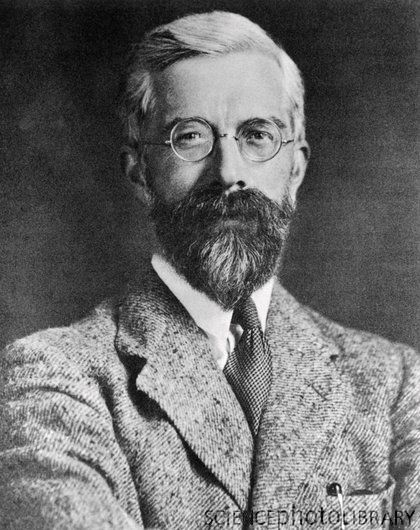
\includegraphics[keepaspectratio]{10_ANOVA_files/mediabag/f193175b503d4d64f7fe.jpg}}\end{footnotesize}}}

A Análise de Variância (ANOVA) é uma das ferramentas estatísticas mais
influentes e amplamente utilizadas \textbf{na comparação de médias entre
grupos}. Seu desenvolvimento é atribuído ao estatístico britânico Ronald
A. Fisher, que a introduziu na década de 1920 como parte de seus
trabalhos pioneiros em experimentação agrícola. Fisher buscava uma forma
eficiente de \textbf{avaliar se diferenças observadas entre médias de
grupos eram estatisticamente significativas ou se poderiam ser
atribuídas apenas à variação aleatória.}

A grande contribuição de Fisher foi estruturar um método baseado na
\textbf{decomposição da variabilidade total dos dados em componentes
atribuíveis a diferentes fontes (como tratamento e erro)}, permitindo
testar hipóteses sobre diferenças entre grupos com base na \textbf{razão
entre essas variâncias}. Desde então, a ANOVA tornou-se essencial em
diversas áreas do conhecimento --- da biologia à engenharia, das
ciências sociais às ciências da saúde --- sempre que se deseja comparar
múltiplos grupos sob um desenho experimental ou observacional
controlado.

\subsection{ANOVA}\label{anova}

Análise de variância com um fator é uma técnica de teste de hipótese
usada para comparar as médias de três ou mais populações. A análise de
variância geralmente é abreviada como ANOVA.

Como mencionado anteriormente, a ANOVA é um teste de razão de
variâncias. O que a estatistica do teste avalia de maneira resumida:

\[Estatística \ do \ Teste = \frac{Variância \ dentro \ dos \ grupos}{Variância \ entre \ grupos}\]

A variância entre as amostras mede as diferenças relacionadas ao
tratamento/efeito atuando em cada amostra. Essa variância também é
conhecida como \textbf{Quadrado Médio do Tratamento}.

Já a variância dentro das amostras mede as diferenças dentro da amostra,
geralmente relacionadas com o erro amostral. Essa variância também é
chamada de \textbf{Quadrado Médio do Resíduo}.

A \textbf{Estatística \(F\)} é o quociente destas duas variâncias, e
nossa hipótese nula na ANOVA testa se a média dos grupos é igual:

\[\large H_0: \mu_1 = \mu_2 = \cdots \mu_n\]

\subsection{Tabela da ANOVA}\label{tabela-da-anova}

\begin{table}
\fontsize{12.0pt}{14.4pt}\selectfont
\begin{tabular*}{0.9\linewidth}{@{\extracolsep{\fill}}ccccc}
\toprule
\textbf{Fontes de Variação (FV)} & \textbf{Graus de Liberdade (GL)} & \textbf{Soma de Quadrados (SQ)} & \textbf{Quadrado Médio (QM)} & \emph{\textbf{F}} \\ 
\midrule\addlinespace[2.5pt]
{Tratamento(entre)} & {\(p-1\)} & {\(SQ_{Trat}\)} & {\(\frac{SQ_{Trat}}{p-1}\)} & {\(\frac{QM_{Trat}}{QM_{Res}}\)} \\ 
{Erro Experimental(dentro)} & {\(n-p\)} & {\(SQ_{Res}\)} & {\(\frac{SQ_{Res}}{n-p}\)} & {} \\ 
{\textbf{Total}} & {\(n-1\)} & {\(SQ_{Total}\)} & {} & {} \\ 
\bottomrule
\end{tabular*}
\end{table}

Esta é a famosa tabela da ANOVA, a mesma tabela que é retornada pelas
funções que utilizaremos aqui no R. As somas de quadrado podem ser
obtidas como:

\(\small \displaystyle SQ_{Total} = \sum_{i=1,j=1}^{I,J}Y_{ij}^2 - \frac{\displaystyle \left( \sum_{i=1,j=1}^{I,J}Y_{ij}\right)^2}{IJ}\)

\(\small \displaystyle SQ_{Trat} = \sum_{i=1}^{I}\frac{T_{i}^2}{J} - \frac{\displaystyle \left( \sum_{i=1,j=1}^{I,J}Y_{ij}\right)^2}{IJ}\)

\(\small SQ_{Total} \ = \ SQ_{Trat} + SQ_{Res}\)

\textbf{Premissas da ANOVA}:

\begin{enumerate}
\def\labelenumi{\arabic{enumi}.}
\tightlist
\item
  As amostras devem ser independentes
\item
  As unidades amostrais são selecionadas aleatoriamente
\item
  Distribuição normal (gaussiana) dos resíduos
\item
  Homogeneidade da variância
\end{enumerate}

\subsection{Anova de um Fator}\label{anova-de-um-fator}

Para nossos exemplos práticos vamos utilizar os dados do pacote
\texttt{palmerpenguins}. São dados morfométricos de diferentes espécies
de pinguins coletados em diferentes ilhas.

Na ANOVA de um fator testamos o efeito de uma única variável categórica
(Tratamento) sobre nossa variável dependente (\(y\)).

\textbf{Pergunta}: Existe diferença no tamanho do bico
(\texttt{bill\_length\_mm}) entre as diferentes espécies de pinguim?

\begin{Shaded}
\begin{Highlighting}[]
\NormalTok{pinguins }\OtherTok{\textless{}{-}}\NormalTok{ palmerpenguins}\SpecialCharTok{::}\NormalTok{penguins}

\NormalTok{pinguins }\SpecialCharTok{|\textgreater{}}
  \FunctionTok{head}\NormalTok{()}
\end{Highlighting}
\end{Shaded}

\begin{verbatim}
# A tibble: 6 x 8
  species island    bill_length_mm bill_depth_mm flipper_length_mm body_mass_g
  <fct>   <fct>              <dbl>         <dbl>             <int>       <int>
1 Adelie  Torgersen           39.1          18.7               181        3750
2 Adelie  Torgersen           39.5          17.4               186        3800
3 Adelie  Torgersen           40.3          18                 195        3250
4 Adelie  Torgersen           NA            NA                  NA          NA
5 Adelie  Torgersen           36.7          19.3               193        3450
6 Adelie  Torgersen           39.3          20.6               190        3650
# i 2 more variables: sex <fct>, year <int>
\end{verbatim}

Diferente da última sessão, utilizaremos a função \texttt{aov()} para
realizarmos a ANOVA.

\begin{Shaded}
\begin{Highlighting}[]
\NormalTok{anova\_bico }\OtherTok{\textless{}{-}} \FunctionTok{aov}\NormalTok{(bill\_length\_mm }\SpecialCharTok{\textasciitilde{}}\NormalTok{ species, }\AttributeTok{data =}\NormalTok{ pinguins)}
\end{Highlighting}
\end{Shaded}

\subsubsection{Testando Premissas}\label{testando-premissas}

Assim como fizemos com nosso modelo de regressão linear podemos avaliar
nossos resíduos visualmente.

\begin{Shaded}
\begin{Highlighting}[]
\FunctionTok{par}\NormalTok{(}\AttributeTok{mfrow =} \FunctionTok{c}\NormalTok{(}\DecValTok{2}\NormalTok{, }\DecValTok{2}\NormalTok{), }\AttributeTok{oma =} \FunctionTok{c}\NormalTok{(}\DecValTok{0}\NormalTok{, }\DecValTok{0}\NormalTok{, }\DecValTok{2}\NormalTok{, }\DecValTok{0}\NormalTok{))}
\FunctionTok{plot}\NormalTok{(anova\_bico)}
\end{Highlighting}
\end{Shaded}

\pandocbounded{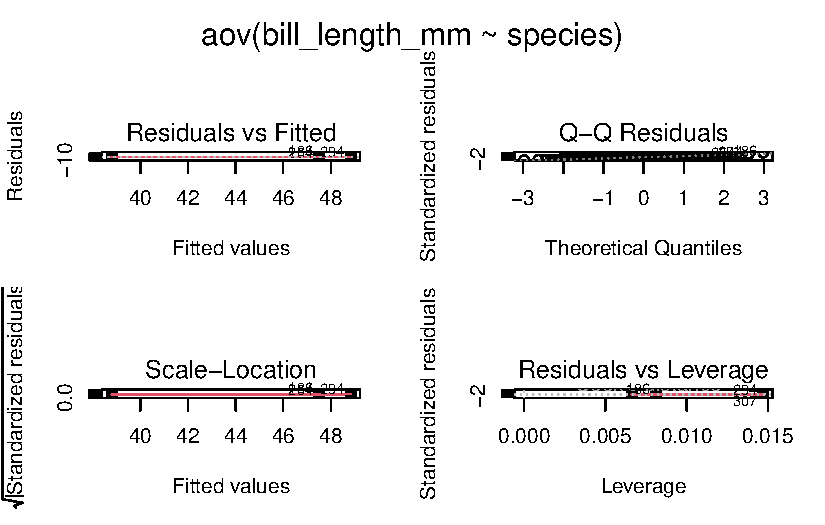
\includegraphics[keepaspectratio]{10_ANOVA_files/figure-pdf/unnamed-chunk-5-1.pdf}}

Nossos resíduos parecem seguir normalidade e homocedasticidade. Mas
podemos confirmar realizando os testes de Shapiro-Wilk (normalidade) e
Bartlett (homocedasticidade).

\faIcon{circle-exclamation} \textbf{Lembre-se que sempre testamos os
resíduos!}

\begin{Shaded}
\begin{Highlighting}[]
\FunctionTok{shapiro.test}\NormalTok{(}\FunctionTok{residuals}\NormalTok{(anova\_bico))}
\end{Highlighting}
\end{Shaded}

\begin{verbatim}

    Shapiro-Wilk normality test

data:  residuals(anova_bico)
W = 0.98903, p-value = 0.01131
\end{verbatim}

\begin{Shaded}
\begin{Highlighting}[]
\FunctionTok{bartlett.test}\NormalTok{(bill\_length\_mm }\SpecialCharTok{\textasciitilde{}}\NormalTok{ species, }\AttributeTok{data =}\NormalTok{ pinguins)}
\end{Highlighting}
\end{Shaded}

\begin{verbatim}

    Bartlett test of homogeneity of variances

data:  bill_length_mm by species
Bartlett's K-squared = 5.6179, df = 2, p-value = 0.06027
\end{verbatim}

Lembrando que a hipótese nula em ambos os testes é de que os dados
seguem normalidade/homocedasticidade. Confirmamos assim o nosso
diagnístico visual.

\subsubsection{Tabela Anova}\label{tabela-anova}

\begin{Shaded}
\begin{Highlighting}[]
\FunctionTok{summary}\NormalTok{(anova\_bico)}
\end{Highlighting}
\end{Shaded}

\begin{verbatim}
             Df Sum Sq Mean Sq F value Pr(>F)    
species       2   7194    3597   410.6 <2e-16 ***
Residuals   339   2970       9                   
---
Signif. codes:  0 '***' 0.001 '**' 0.01 '*' 0.05 '.' 0.1 ' ' 1
2 observations deleted due to missingness
\end{verbatim}

E aqui obtemos a nossa tabela da ANOVA. E com base no p-valor obtido
podemos confirmar que existe efeito de Espécie sobre o Tamanho do Bico
dos Pinguins. Em relação a nossa hipótese nula, isso significa dizer que
\textbf{pelo menos um dos grupos avaliados possui média diferente dos
demais}.

\subsubsection{Comparação de
Médias}\label{comparauxe7uxe3o-de-muxe9dias}

Uma vez sabendo que existe diferença significativa, agora precisamos
realizar um pós-teste de comparação de médias entre os grupos. Para isso
vamos utilizar o pacote \texttt{agricolae}. Este pacote é excelente por
possuir diversos pos-testes para anova, entre eles Tukey, SNK, e Duncan.

\subsubsection{Tukey HSD}\label{tukey-hsd}

O Teste \textbf{Tukey HSD (\emph{honestly significant difference})} é
amplamente reconhecido por controlar de forma rigorosa a taxa de erro
familiar, permitindo comparações par a par entre todas as médias com um
critério bastante robusto.

\begin{Shaded}
\begin{Highlighting}[]
\NormalTok{agricolae}\SpecialCharTok{::}\FunctionTok{HSD.test}\NormalTok{(anova\_bico,}\StringTok{"species"}\NormalTok{, }\AttributeTok{group=}\ConstantTok{TRUE}\NormalTok{, }\AttributeTok{console=}\ConstantTok{TRUE}\NormalTok{)}
\end{Highlighting}
\end{Shaded}

\begin{verbatim}

Study: anova_bico ~ "species"

HSD Test for bill_length_mm 

Mean Square Error:  8.760732 

species,  means

          bill_length_mm      std   r        se  Min  Max   Q25   Q50    Q75
Adelie          38.79139 2.663405 151 0.2408694 32.1 46.0 36.75 38.80 40.750
Chinstrap       48.83382 3.339256  68 0.3589349 40.9 58.0 46.35 49.55 51.075
Gentoo          47.50488 3.081857 123 0.2668810 40.9 59.6 45.30 47.30 49.550

Alpha: 0.05 ; DF Error: 339 
Critical Value of Studentized Range: 3.329136 

Groups according to probability of means differences and alpha level( 0.05 )

Treatments with the same letter are not significantly different.

          bill_length_mm groups
Chinstrap       48.83382      a
Gentoo          47.50488      b
Adelie          38.79139      c
\end{verbatim}

\subsubsection{SNK}\label{snk}

O Teste \textbf{Student-Newman-Keuls (SNK)} realiza comparações par a
par de maneira sequencial, equilibrando a sensibilidade para detectar
diferenças com um critério menos conservador que o Tukey HSD, mas mais
rigoroso que o teste de Duncan.

\begin{Shaded}
\begin{Highlighting}[]
\NormalTok{agricolae}\SpecialCharTok{::}\FunctionTok{SNK.test}\NormalTok{(anova\_bico, }\StringTok{"species"}\NormalTok{, }\AttributeTok{group =} \ConstantTok{TRUE}\NormalTok{, }\AttributeTok{console =} \ConstantTok{TRUE}\NormalTok{)}
\end{Highlighting}
\end{Shaded}

\begin{verbatim}

Study: anova_bico ~ "species"

Student Newman Keuls Test
for bill_length_mm 

Mean Square Error:  8.760732 

species,  means

          bill_length_mm      std   r        se  Min  Max   Q25   Q50    Q75
Adelie          38.79139 2.663405 151 0.2408694 32.1 46.0 36.75 38.80 40.750
Chinstrap       48.83382 3.339256  68 0.3589349 40.9 58.0 46.35 49.55 51.075
Gentoo          47.50488 3.081857 123 0.2668810 40.9 59.6 45.30 47.30 49.550

Groups according to probability of means differences and alpha level( 0.05 )

Means with the same letter are not significantly different.

          bill_length_mm groups
Chinstrap       48.83382      a
Gentoo          47.50488      b
Adelie          38.79139      c
\end{verbatim}

\subsubsection{Duncan}\label{duncan}

O Teste de \textbf{Duncan} adota uma abordagem mais liberal, facilitando
a identificação de intervalos de similaridade entre as médias, mas com
uma margem maior de risco de erro do Tipo I.

\begin{Shaded}
\begin{Highlighting}[]
\NormalTok{agricolae}\SpecialCharTok{::}\FunctionTok{duncan.test}\NormalTok{(anova\_bico, }\StringTok{"species"}\NormalTok{, }\AttributeTok{group =} \ConstantTok{TRUE}\NormalTok{, }\AttributeTok{console =} \ConstantTok{TRUE}\NormalTok{)}
\end{Highlighting}
\end{Shaded}

\begin{verbatim}

Study: anova_bico ~ "species"

Duncan's new multiple range test
for bill_length_mm 

Mean Square Error:  8.760732 

species,  means

          bill_length_mm      std   r        se  Min  Max   Q25   Q50    Q75
Adelie          38.79139 2.663405 151 0.2408694 32.1 46.0 36.75 38.80 40.750
Chinstrap       48.83382 3.339256  68 0.3589349 40.9 58.0 46.35 49.55 51.075
Gentoo          47.50488 3.081857 123 0.2668810 40.9 59.6 45.30 47.30 49.550

Groups according to probability of means differences and alpha level( 0.05 )

Means with the same letter are not significantly different.

          bill_length_mm groups
Chinstrap       48.83382      a
Gentoo          47.50488      b
Adelie          38.79139      c
\end{verbatim}

\subsubsection{Dunnet}\label{dunnet}

O Teste \textbf{Dunnett} é particularmente útil quando o objetivo
principal é comparar cada tratamento com um grupo de controle, focando
essa análise e ajustando as comparações para esse propósito.

Para realizar esse teste usaremos o pacote \texttt{multcomp}.

\begin{Shaded}
\begin{Highlighting}[]
\NormalTok{multcomp}\SpecialCharTok{::}\FunctionTok{glht}\NormalTok{(anova\_bico, }\AttributeTok{linfct =}\NormalTok{ multcomp}\SpecialCharTok{::}\FunctionTok{mcp}\NormalTok{(}\AttributeTok{species=} \StringTok{"Dunnett"}\NormalTok{))}
\end{Highlighting}
\end{Shaded}

\begin{verbatim}

     General Linear Hypotheses

Multiple Comparisons of Means: Dunnett Contrasts


Linear Hypotheses:
                        Estimate
Chinstrap - Adelie == 0   10.042
Gentoo - Adelie == 0       8.713
\end{verbatim}

\subsubsection{Apresentando os
resultados}\label{apresentando-os-resultados}




\end{document}
